\documentclass[1p]{elsarticle_modified}
%\bibliographystyle{elsarticle-num}

%\usepackage[colorlinks]{hyperref}
%\usepackage{abbrmath_seonhwa} %\Abb, \Ascr, \Acal ,\Abf, \Afrak
\usepackage{amsfonts}
\usepackage{amssymb}
\usepackage{amsmath}
\usepackage{amsthm}
\usepackage{scalefnt}
\usepackage{amsbsy}
\usepackage{kotex}
\usepackage{caption}
\usepackage{subfig}
\usepackage{color}
\usepackage{graphicx}
\usepackage{xcolor} %% white, black, red, green, blue, cyan, magenta, yellow
\usepackage{float}
\usepackage{setspace}
\usepackage{hyperref}

\usepackage{tikz}
\usetikzlibrary{arrows}

\usepackage{multirow}
\usepackage{array} % fixed length table
\usepackage{hhline}

%%%%%%%%%%%%%%%%%%%%%
\makeatletter
\renewcommand*\env@matrix[1][\arraystretch]{%
	\edef\arraystretch{#1}%
	\hskip -\arraycolsep
	\let\@ifnextchar\new@ifnextchar
	\array{*\c@MaxMatrixCols c}}
\makeatother %https://tex.stackexchange.com/questions/14071/how-can-i-increase-the-line-spacing-in-a-matrix
%%%%%%%%%%%%%%%

\usepackage[normalem]{ulem}

\newcommand{\msout}[1]{\ifmmode\text{\sout{\ensuremath{#1}}}\else\sout{#1}\fi}
%SOURCE: \msout is \stkout macro in https://tex.stackexchange.com/questions/20609/strikeout-in-math-mode

\newcommand{\cancel}[1]{
	\ifmmode
	{\color{red}\msout{#1}}
	\else
	{\color{red}\sout{#1}}
	\fi
}

\newcommand{\add}[1]{
	{\color{blue}\uwave{#1}}
}

\newcommand{\replace}[2]{
	\ifmmode
	{\color{red}\msout{#1}}{\color{blue}\uwave{#2}}
	\else
	{\color{red}\sout{#1}}{\color{blue}\uwave{#2}}
	\fi
}

\newcommand{\Sol}{\mathcal{S}} %segment
\newcommand{\D}{D} %diagram
\newcommand{\A}{\mathcal{A}} %arc


%%%%%%%%%%%%%%%%%%%%%%%%%%%%%5 test

\def\sl{\operatorname{\textup{SL}}(2,\Cbb)}
\def\psl{\operatorname{\textup{PSL}}(2,\Cbb)}
\def\quan{\mkern 1mu \triangleright \mkern 1mu}

\theoremstyle{definition}
\newtheorem{thm}{Theorem}[section]
\newtheorem{prop}[thm]{Proposition}
\newtheorem{lem}[thm]{Lemma}
\newtheorem{ques}[thm]{Question}
\newtheorem{cor}[thm]{Corollary}
\newtheorem{defn}[thm]{Definition}
\newtheorem{exam}[thm]{Example}
\newtheorem{rmk}[thm]{Remark}
\newtheorem{alg}[thm]{Algorithm}

\newcommand{\I}{\sqrt{-1}}
\begin{document}

%\begin{frontmatter}
%
%\title{Boundary parabolic representations of knots up to 8 crossings}
%
%%% Group authors per affiliation:
%\author{Yunhi Cho} 
%\address{Department of Mathematics, University of Seoul, Seoul, Korea}
%\ead{yhcho@uos.ac.kr}
%
%
%\author{Seonhwa Kim} %\fnref{s_kim}}
%\address{Center for Geometry and Physics, Institute for Basic Science, Pohang, 37673, Korea}
%\ead{ryeona17@ibs.re.kr}
%
%\author{Hyuk Kim}
%\address{Department of Mathematical Sciences, Seoul National University, Seoul 08826, Korea}
%\ead{hyukkim@snu.ac.kr}
%
%\author{Seokbeom Yoon}
%\address{Department of Mathematical Sciences, Seoul National University, Seoul, 08826,  Korea}
%\ead{sbyoon15@snu.ac.kr}
%
%\begin{abstract}
%We find all boundary parabolic representation of knots up to 8 crossings.
%
%\end{abstract}
%\begin{keyword}
%    \MSC[2010] 57M25 
%\end{keyword}
%
%\end{frontmatter}

%\linenumbers
%\tableofcontents
%
\newcommand\colored[1]{\textcolor{white}{\rule[-0.35ex]{0.8em}{1.4ex}}\kern-0.8em\color{red} #1}%
%\newcommand\colored[1]{\textcolor{white}{ #1}\kern-2.17ex	\textcolor{white}{ #1}\kern-1.81ex	\textcolor{white}{ #1}\kern-2.15ex\color{red}#1	}

{\Large $\underline{12n_{0150}~(K12n_{0150})}$}

\setlength{\tabcolsep}{10pt}
\renewcommand{\arraystretch}{1.6}
\vspace{1cm}\begin{tabular}{m{100pt}>{\centering\arraybackslash}m{274pt}}
\multirow{5}{120pt}{
	\centering
	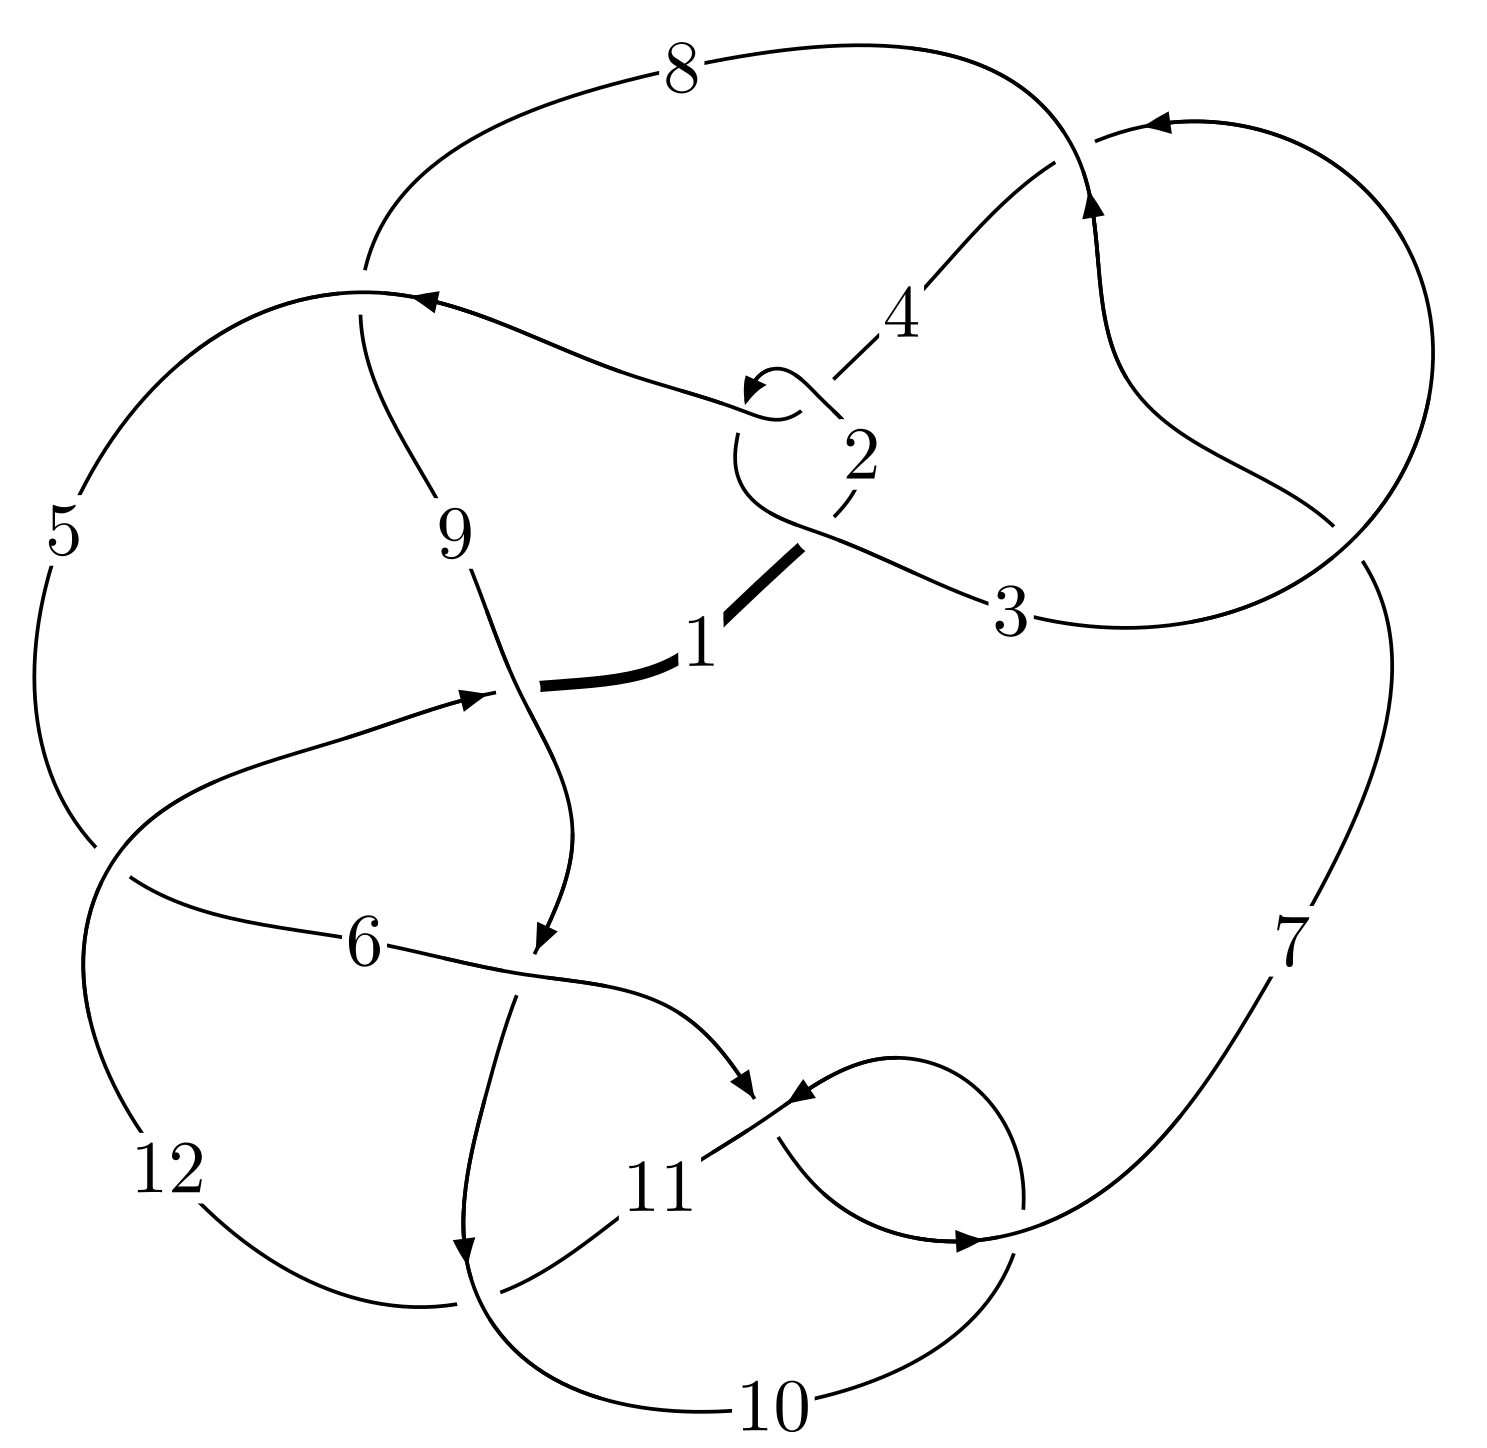
\includegraphics[width=112pt]{../../../GIT/diagram.site/Diagrams/png/2239_12n_0150.png}\\
\ \ \ A knot diagram\footnotemark}&
\allowdisplaybreaks
\textbf{Linearized knot diagam} \\
\cline{2-2}
 &
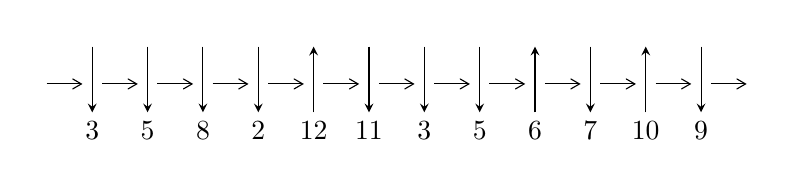
\begin{tikzpicture}[x=20pt, y=17pt]
	% nodes
	\node (C0) at (0, 0) {};
	\node (C1) at (1, 0) {};
	\node (C1U) at (1, +1) {};
	\node (C1D) at (1, -1) {3};

	\node (C2) at (2, 0) {};
	\node (C2U) at (2, +1) {};
	\node (C2D) at (2, -1) {5};

	\node (C3) at (3, 0) {};
	\node (C3U) at (3, +1) {};
	\node (C3D) at (3, -1) {8};

	\node (C4) at (4, 0) {};
	\node (C4U) at (4, +1) {};
	\node (C4D) at (4, -1) {2};

	\node (C5) at (5, 0) {};
	\node (C5U) at (5, +1) {};
	\node (C5D) at (5, -1) {12};

	\node (C6) at (6, 0) {};
	\node (C6U) at (6, +1) {};
	\node (C6D) at (6, -1) {11};

	\node (C7) at (7, 0) {};
	\node (C7U) at (7, +1) {};
	\node (C7D) at (7, -1) {3};

	\node (C8) at (8, 0) {};
	\node (C8U) at (8, +1) {};
	\node (C8D) at (8, -1) {5};

	\node (C9) at (9, 0) {};
	\node (C9U) at (9, +1) {};
	\node (C9D) at (9, -1) {6};

	\node (C10) at (10, 0) {};
	\node (C10U) at (10, +1) {};
	\node (C10D) at (10, -1) {7};

	\node (C11) at (11, 0) {};
	\node (C11U) at (11, +1) {};
	\node (C11D) at (11, -1) {10};

	\node (C12) at (12, 0) {};
	\node (C12U) at (12, +1) {};
	\node (C12D) at (12, -1) {9};
	\node (C13) at (13, 0) {};

	% arrows
	\draw[->,>={angle 60}]
	(C0) edge (C1) (C1) edge (C2) (C2) edge (C3) (C3) edge (C4) (C4) edge (C5) (C5) edge (C6) (C6) edge (C7) (C7) edge (C8) (C8) edge (C9) (C9) edge (C10) (C10) edge (C11) (C11) edge (C12) (C12) edge (C13) ;	\draw[->,>=stealth]
	(C1U) edge (C1D) (C2U) edge (C2D) (C3U) edge (C3D) (C4U) edge (C4D) (C5D) edge (C5U) (C6U) edge (C6D) (C7U) edge (C7D) (C8U) edge (C8D) (C9D) edge (C9U) (C10U) edge (C10D) (C11D) edge (C11U) (C12U) edge (C12D) ;
	\end{tikzpicture} \\
\hhline{~~} \\& 
\textbf{Solving Sequence} \\ \cline{2-2} 
 &
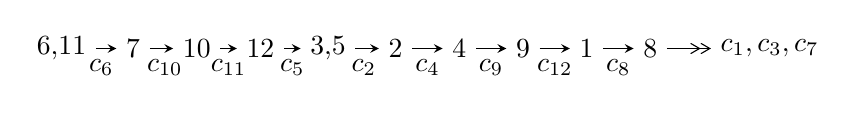
\begin{tikzpicture}[x=23pt, y=7pt]
	% node
	\node (A0) at (-1/8, 0) {6,11};
	\node (A1) at (1, 0) {7};
	\node (A2) at (2, 0) {10};
	\node (A3) at (3, 0) {12};
	\node (A4) at (65/16, 0) {3,5};
	\node (A5) at (41/8, 0) {2};
	\node (A6) at (49/8, 0) {4};
	\node (A7) at (57/8, 0) {9};
	\node (A8) at (65/8, 0) {1};
	\node (A9) at (73/8, 0) {8};
	\node (C1) at (1/2, -1) {$c_{6}$};
	\node (C2) at (3/2, -1) {$c_{10}$};
	\node (C3) at (5/2, -1) {$c_{11}$};
	\node (C4) at (7/2, -1) {$c_{5}$};
	\node (C5) at (37/8, -1) {$c_{2}$};
	\node (C6) at (45/8, -1) {$c_{4}$};
	\node (C7) at (53/8, -1) {$c_{9}$};
	\node (C8) at (61/8, -1) {$c_{12}$};
	\node (C9) at (69/8, -1) {$c_{8}$};
	\node (A10) at (11, 0) {$c_{1},c_{3},c_{7}$};

	% edge
	\draw[->,>=stealth]	
	(A0) edge (A1) (A1) edge (A2) (A2) edge (A3) (A3) edge (A4) (A4) edge (A5) (A5) edge (A6) (A6) edge (A7) (A7) edge (A8) (A8) edge (A9) ;
	\draw[->>,>={angle 60}]	
	(A9) edge (A10);
\end{tikzpicture} \\ 

\end{tabular} \\

\footnotetext{
The image of knot diagram is generated by the software ``\textbf{Draw programme}" developed by Andrew Bartholomew(\url{http://www.layer8.co.uk/maths/draw/index.htm\#Running-draw}), where we modified some parts for our purpose(\url{https://github.com/CATsTAILs/LinksPainter}).
}\phantom \\ \newline 
\centering \textbf{Ideals for irreducible components\footnotemark of $X_{\text{par}}$} 
 
\begin{align*}
I^u_{1}&=\langle 
u^{36}- u^{35}+\cdots+b-2 u,\;- u^{36}+u^{35}+\cdots+a+1,\;u^{38}-2 u^{37}+\cdots-5 u+1\rangle \\
I^u_{2}&=\langle 
b+u,\;- u^3+a- u+1,\;u^4+u^2- u+1\rangle \\
I^u_{3}&=\langle 
- u^5- u^4-2 u^3-2 u^2+b-2 u-1,\;u^4+u^2+a,\;u^6+u^5+2 u^4+2 u^3+2 u^2+2 u+1\rangle \\
\\
\end{align*}
\raggedright * 3 irreducible components of $\dim_{\mathbb{C}}=0$, with total 48 representations.\\
\footnotetext{All coefficients of polynomials are rational numbers. But the coefficients are sometimes approximated in decimal forms when there is not enough margin.}
\newpage
\renewcommand{\arraystretch}{1}
\centering \section*{I. $I^u_{1}= \langle u^{36}- u^{35}+\cdots+b-2 u,\;- u^{36}+u^{35}+\cdots+a+1,\;u^{38}-2 u^{37}+\cdots-5 u+1 \rangle$}
\flushleft \textbf{(i) Arc colorings}\\
\begin{tabular}{m{7pt} m{180pt} m{7pt} m{180pt} }
\flushright $a_{6}=$&$\begin{pmatrix}1\\0\end{pmatrix}$ \\
\flushright $a_{11}=$&$\begin{pmatrix}0\\u\end{pmatrix}$ \\
\flushright $a_{7}=$&$\begin{pmatrix}1\\u^2\end{pmatrix}$ \\
\flushright $a_{10}=$&$\begin{pmatrix}u\\u^3+u\end{pmatrix}$ \\
\flushright $a_{12}=$&$\begin{pmatrix}u^3\\u^5+u^3+u\end{pmatrix}$ \\
\flushright $a_{3}=$&$\begin{pmatrix}u^{36}- u^{35}+\cdots-2 u^3-1\\- u^{36}+u^{35}+\cdots-3 u^2+2 u\end{pmatrix}$ \\
\flushright $a_{5}=$&$\begin{pmatrix}u^8+u^6+u^4+1\\u^{10}+2 u^8+3 u^6+2 u^4+u^2\end{pmatrix}$ \\
\flushright $a_{2}=$&$\begin{pmatrix}- u^{34}+u^{33}+\cdots+3 u-1\\- u^{36}+u^{35}+\cdots-2 u^2+2 u\end{pmatrix}$ \\
\flushright $a_{4}=$&$\begin{pmatrix}u^{36}- u^{35}+\cdots-4 u+2\\- u^{36}- u^{35}+\cdots+u^2- u\end{pmatrix}$ \\
\flushright $a_{9}=$&$\begin{pmatrix}- u^3\\u^3+u\end{pmatrix}$ \\
\flushright $a_{1}=$&$\begin{pmatrix}- u^{11}-2 u^9-2 u^7+u^3\\u^{11}+3 u^9+4 u^7+3 u^5+u^3+u\end{pmatrix}$ \\
\flushright $a_{8}=$&$\begin{pmatrix}u^{21}+4 u^{19}+9 u^{17}+12 u^{15}+12 u^{13}+10 u^{11}+9 u^9+6 u^7+3 u^5+u\\u^{23}+5 u^{21}+\cdots+2 u^3+u\end{pmatrix}$\\&\end{tabular}
\flushleft \textbf{(ii) Obstruction class $= -1$}\\~\\
\flushleft \textbf{(iii) Cusp Shapes $= 4 u^{37}-12 u^{36}+46 u^{35}-104 u^{34}+244 u^{33}-468 u^{32}+837 u^{31}-1403 u^{30}+2076 u^{29}-3097 u^{28}+3974 u^{27}-5326 u^{26}+6111 u^{25}-7416 u^{24}+7798 u^{23}-8645 u^{22}+8473 u^{21}-8673 u^{20}+8000 u^{19}-7644 u^{18}+6639 u^{17}-5962 u^{16}+4886 u^{15}-4146 u^{14}+3236 u^{13}-2602 u^{12}+1976 u^{11}-1512 u^{10}+1108 u^9-780 u^8+540 u^7-353 u^6+237 u^5-147 u^4+100 u^3-62 u^2+37 u-18$}\\~\\
\newpage\renewcommand{\arraystretch}{1}
\flushleft \textbf{(iv) u-Polynomials at the component}\newline \\
\begin{tabular}{m{50pt}|m{274pt}}
Crossings & \hspace{64pt}u-Polynomials at each crossing \\
\hline $$\begin{aligned}c_{1}\end{aligned}$$&$\begin{aligned}
&u^{38}+57 u^{37}+\cdots+4 u+1
\end{aligned}$\\
\hline $$\begin{aligned}c_{2},c_{4}\end{aligned}$$&$\begin{aligned}
&u^{38}-11 u^{37}+\cdots+10 u-1
\end{aligned}$\\
\hline $$\begin{aligned}c_{3},c_{7}\end{aligned}$$&$\begin{aligned}
&u^{38}- u^{37}+\cdots-1024 u-1024
\end{aligned}$\\
\hline $$\begin{aligned}c_{5}\end{aligned}$$&$\begin{aligned}
&u^{38}+10 u^{37}+\cdots+313 u+43
\end{aligned}$\\
\hline $$\begin{aligned}c_{6},c_{10}\end{aligned}$$&$\begin{aligned}
&u^{38}+2 u^{37}+\cdots+5 u+1
\end{aligned}$\\
\hline $$\begin{aligned}c_{8}\end{aligned}$$&$\begin{aligned}
&u^{38}+2 u^{37}+\cdots+3 u+1
\end{aligned}$\\
\hline $$\begin{aligned}c_{9}\end{aligned}$$&$\begin{aligned}
&u^{38}-2 u^{37}+\cdots-24 u+8
\end{aligned}$\\
\hline $$\begin{aligned}c_{11}\end{aligned}$$&$\begin{aligned}
&u^{38}-18 u^{37}+\cdots+5 u+1
\end{aligned}$\\
\hline $$\begin{aligned}c_{12}\end{aligned}$$&$\begin{aligned}
&u^{38}-6 u^{37}+\cdots-2663 u+61
\end{aligned}$\\
\hline
\end{tabular}\\~\\
\newpage\renewcommand{\arraystretch}{1}
\flushleft \textbf{(v) Riley Polynomials at the component}\newline \\
\begin{tabular}{m{50pt}|m{274pt}}
Crossings & \hspace{64pt}Riley Polynomials at each crossing \\
\hline $$\begin{aligned}c_{1}\end{aligned}$$&$\begin{aligned}
&y^{38}-141 y^{37}+\cdots-12 y+1
\end{aligned}$\\
\hline $$\begin{aligned}c_{2},c_{4}\end{aligned}$$&$\begin{aligned}
&y^{38}-57 y^{37}+\cdots-4 y+1
\end{aligned}$\\
\hline $$\begin{aligned}c_{3},c_{7}\end{aligned}$$&$\begin{aligned}
&y^{38}-63 y^{37}+\cdots+8912896 y+1048576
\end{aligned}$\\
\hline $$\begin{aligned}c_{5}\end{aligned}$$&$\begin{aligned}
&y^{38}+18 y^{37}+\cdots+243 y+1849
\end{aligned}$\\
\hline $$\begin{aligned}c_{6},c_{10}\end{aligned}$$&$\begin{aligned}
&y^{38}+18 y^{37}+\cdots-5 y+1
\end{aligned}$\\
\hline $$\begin{aligned}c_{8}\end{aligned}$$&$\begin{aligned}
&y^{38}-78 y^{37}+\cdots-5 y+1
\end{aligned}$\\
\hline $$\begin{aligned}c_{9}\end{aligned}$$&$\begin{aligned}
&y^{38}-6 y^{37}+\cdots-1680 y+64
\end{aligned}$\\
\hline $$\begin{aligned}c_{11}\end{aligned}$$&$\begin{aligned}
&y^{38}+6 y^{37}+\cdots-77 y+1
\end{aligned}$\\
\hline $$\begin{aligned}c_{12}\end{aligned}$$&$\begin{aligned}
&y^{38}-18 y^{37}+\cdots-5705405 y+3721
\end{aligned}$\\
\hline
\end{tabular}\\~\\
\newpage\flushleft \textbf{(vi) Complex Volumes and Cusp Shapes}
$$\begin{array}{c|c|c}  
\text{Solutions to }I^u_{1}& \I (\text{vol} + \sqrt{-1}CS) & \text{Cusp shape}\\
 \hline 
\begin{aligned}
u &= \phantom{-}0.190184 + 1.006430 I \\
a &= \phantom{-}0.666672 + 0.650134 I \\
b &= \phantom{-}0.171965 - 0.057486 I\end{aligned}
 & -0.043597 + 0.941262 I & -5.60914 - 1.60302 I \\ \hline\begin{aligned}
u &= \phantom{-}0.190184 - 1.006430 I \\
a &= \phantom{-}0.666672 - 0.650134 I \\
b &= \phantom{-}0.171965 + 0.057486 I\end{aligned}
 & -0.043597 - 0.941262 I & -5.60914 + 1.60302 I \\ \hline\begin{aligned}
u &= -0.330777 + 0.907409 I \\
a &= \phantom{-}0.06706 + 2.30485 I \\
b &= \phantom{-}1.66441 - 0.88267 I\end{aligned}
 & -0.97161 + 1.42227 I & -5.26135 - 0.25979 I \\ \hline\begin{aligned}
u &= -0.330777 - 0.907409 I \\
a &= \phantom{-}0.06706 - 2.30485 I \\
b &= \phantom{-}1.66441 + 0.88267 I\end{aligned}
 & -0.97161 - 1.42227 I & -5.26135 + 0.25979 I \\ \hline\begin{aligned}
u &= -0.732889 + 0.615448 I \\
a &= -0.77820 - 1.38388 I \\
b &= \phantom{-}0.885934 + 0.086371 I\end{aligned}
 & -16.4068 + 4.3334 I & -12.33818 - 2.98248 I \\ \hline\begin{aligned}
u &= -0.732889 - 0.615448 I \\
a &= -0.77820 + 1.38388 I \\
b &= \phantom{-}0.885934 - 0.086371 I\end{aligned}
 & -16.4068 - 4.3334 I & -12.33818 + 2.98248 I \\ \hline\begin{aligned}
u &= \phantom{-}0.392112 + 1.025700 I \\
a &= -0.398310 - 0.990025 I \\
b &= \phantom{-}0.344483 + 0.379769 I\end{aligned}
 & \phantom{-}1.28562 - 2.93709 I & -3.65871 + 5.49454 I \\ \hline\begin{aligned}
u &= \phantom{-}0.392112 - 1.025700 I \\
a &= -0.398310 + 0.990025 I \\
b &= \phantom{-}0.344483 - 0.379769 I\end{aligned}
 & \phantom{-}1.28562 + 2.93709 I & -3.65871 - 5.49454 I \\ \hline\begin{aligned}
u &= \phantom{-}0.808282 + 0.376060 I \\
a &= -0.308296 - 1.239560 I \\
b &= \phantom{-}2.75261 - 1.36307 I\end{aligned}
 & -15.0919 + 7.2035 I & -11.42537 - 2.83717 I \\ \hline\begin{aligned}
u &= \phantom{-}0.808282 - 0.376060 I \\
a &= -0.308296 + 1.239560 I \\
b &= \phantom{-}2.75261 + 1.36307 I\end{aligned}
 & -15.0919 - 7.2035 I & -11.42537 + 2.83717 I\\
 \hline 
 \end{array}$$\newpage$$\begin{array}{c|c|c}  
\text{Solutions to }I^u_{1}& \I (\text{vol} + \sqrt{-1}CS) & \text{Cusp shape}\\
 \hline 
\begin{aligned}
u &= -0.283537 + 1.096170 I \\
a &= -0.116887 - 1.308640 I \\
b &= -0.749932 + 0.972888 I\end{aligned}
 & \phantom{-}3.86766 + 0.18519 I & \phantom{-}3.63146 - 0.12416 I \\ \hline\begin{aligned}
u &= -0.283537 - 1.096170 I \\
a &= -0.116887 + 1.308640 I \\
b &= -0.749932 - 0.972888 I\end{aligned}
 & \phantom{-}3.86766 - 0.18519 I & \phantom{-}3.63146 + 0.12416 I \\ \hline\begin{aligned}
u &= -0.694068 + 0.485559 I \\
a &= \phantom{-}1.073670 - 0.121248 I \\
b &= -0.86069 - 1.59817 I\end{aligned}
 & -4.83970 + 0.46505 I & -12.83571 - 0.64239 I \\ \hline\begin{aligned}
u &= -0.694068 - 0.485559 I \\
a &= \phantom{-}1.073670 + 0.121248 I \\
b &= -0.86069 + 1.59817 I\end{aligned}
 & -4.83970 - 0.46505 I & -12.83571 + 0.64239 I \\ \hline\begin{aligned}
u &= \phantom{-}0.725358 + 0.427516 I \\
a &= \phantom{-}0.910150 + 0.189413 I \\
b &= -1.062290 + 0.018396 I\end{aligned}
 & -4.53414 + 2.77322 I & -12.23678 - 1.99066 I \\ \hline\begin{aligned}
u &= \phantom{-}0.725358 - 0.427516 I \\
a &= \phantom{-}0.910150 - 0.189413 I \\
b &= -1.062290 - 0.018396 I\end{aligned}
 & -4.53414 - 2.77322 I & -12.23678 + 1.99066 I \\ \hline\begin{aligned}
u &= \phantom{-}0.520749 + 1.037540 I \\
a &= -0.591726 - 0.036334 I \\
b &= -0.0031098 - 0.1233600 I\end{aligned}
 & \phantom{-}0.43968 - 3.37790 I & -4.33141 + 2.37402 I \\ \hline\begin{aligned}
u &= \phantom{-}0.520749 - 1.037540 I \\
a &= -0.591726 + 0.036334 I \\
b &= -0.0031098 + 0.1233600 I\end{aligned}
 & \phantom{-}0.43968 + 3.37790 I & -4.33141 - 2.37402 I \\ \hline\begin{aligned}
u &= -0.635679 + 0.975329 I \\
a &= -0.60721 + 1.51515 I \\
b &= -0.083609 - 0.380918 I\end{aligned}
 & -15.3384 + 0.8717 I & -10.72381 - 2.45601 I \\ \hline\begin{aligned}
u &= -0.635679 - 0.975329 I \\
a &= -0.60721 - 1.51515 I \\
b &= -0.083609 + 0.380918 I\end{aligned}
 & -15.3384 - 0.8717 I & -10.72381 + 2.45601 I\\
 \hline 
 \end{array}$$\newpage$$\begin{array}{c|c|c}  
\text{Solutions to }I^u_{1}& \I (\text{vol} + \sqrt{-1}CS) & \text{Cusp shape}\\
 \hline 
\begin{aligned}
u &= \phantom{-}0.169305 + 1.157370 I \\
a &= -2.96351 + 1.28333 I \\
b &= \phantom{-}1.31226 - 2.38449 I\end{aligned}
 & -10.03480 + 4.57409 I & -5.57316 - 1.67266 I \\ \hline\begin{aligned}
u &= \phantom{-}0.169305 - 1.157370 I \\
a &= -2.96351 - 1.28333 I \\
b &= \phantom{-}1.31226 + 2.38449 I\end{aligned}
 & -10.03480 - 4.57409 I & -5.57316 + 1.67266 I \\ \hline\begin{aligned}
u &= -0.578647 + 1.054140 I \\
a &= -1.47418 - 2.16069 I \\
b &= -0.53165 + 2.48877 I\end{aligned}
 & -3.15884 + 4.44653 I & -9.57300 - 4.70180 I \\ \hline\begin{aligned}
u &= -0.578647 - 1.054140 I \\
a &= -1.47418 + 2.16069 I \\
b &= -0.53165 - 2.48877 I\end{aligned}
 & -3.15884 - 4.44653 I & -9.57300 + 4.70180 I \\ \hline\begin{aligned}
u &= -0.698518 + 0.329444 I \\
a &= -0.420323 + 0.439871 I \\
b &= \phantom{-}0.191136 + 0.950537 I\end{aligned}
 & -0.20642 - 2.47480 I & -3.77716 + 2.78494 I \\ \hline\begin{aligned}
u &= -0.698518 - 0.329444 I \\
a &= -0.420323 - 0.439871 I \\
b &= \phantom{-}0.191136 - 0.950537 I\end{aligned}
 & -0.20642 + 2.47480 I & -3.77716 - 2.78494 I \\ \hline\begin{aligned}
u &= \phantom{-}0.581924 + 1.085040 I \\
a &= \phantom{-}0.77887 + 1.33818 I \\
b &= -0.985828 - 0.678181 I\end{aligned}
 & -2.59793 - 7.77172 I & -8.83321 + 6.58917 I \\ \hline\begin{aligned}
u &= \phantom{-}0.581924 - 1.085040 I \\
a &= \phantom{-}0.77887 - 1.33818 I \\
b &= -0.985828 + 0.678181 I\end{aligned}
 & -2.59793 + 7.77172 I & -8.83321 - 6.58917 I \\ \hline\begin{aligned}
u &= \phantom{-}0.561548 + 0.523699 I \\
a &= -0.514245 + 0.265142 I \\
b &= \phantom{-}0.143026 + 0.191094 I\end{aligned}
 & -1.11182 - 0.98490 I & -6.72845 + 3.76025 I \\ \hline\begin{aligned}
u &= \phantom{-}0.561548 - 0.523699 I \\
a &= -0.514245 - 0.265142 I \\
b &= \phantom{-}0.143026 - 0.191094 I\end{aligned}
 & -1.11182 + 0.98490 I & -6.72845 - 3.76025 I\\
 \hline 
 \end{array}$$\newpage$$\begin{array}{c|c|c}  
\text{Solutions to }I^u_{1}& \I (\text{vol} + \sqrt{-1}CS) & \text{Cusp shape}\\
 \hline 
\begin{aligned}
u &= \phantom{-}0.424583 + 1.162280 I \\
a &= \phantom{-}3.07997 + 1.73117 I \\
b &= -3.42587 + 1.10441 I\end{aligned}
 & -6.91800 - 4.12327 I & -5.26243 + 3.48548 I \\ \hline\begin{aligned}
u &= \phantom{-}0.424583 - 1.162280 I \\
a &= \phantom{-}3.07997 - 1.73117 I \\
b &= -3.42587 - 1.10441 I\end{aligned}
 & -6.91800 + 4.12327 I & -5.26243 - 3.48548 I \\ \hline\begin{aligned}
u &= -0.549992 + 1.111450 I \\
a &= \phantom{-}0.916076 + 1.068210 I \\
b &= \phantom{-}0.33127 - 1.48940 I\end{aligned}
 & \phantom{-}2.05645 + 7.27341 I & -0.29909 - 6.10879 I \\ \hline\begin{aligned}
u &= -0.549992 - 1.111450 I \\
a &= \phantom{-}0.916076 - 1.068210 I \\
b &= \phantom{-}0.33127 + 1.48940 I\end{aligned}
 & \phantom{-}2.05645 - 7.27341 I & -0.29909 + 6.10879 I \\ \hline\begin{aligned}
u &= \phantom{-}0.738732\phantom{ +0.000000I} \\
a &= -1.26309\phantom{ +0.000000I} \\
b &= -2.66464\phantom{ +0.000000I}\end{aligned}
 & -10.3080\phantom{ +0.000000I} & -9.27210\phantom{ +0.000000I} \\ \hline\begin{aligned}
u &= \phantom{-}0.596983 + 1.127320 I \\
a &= -0.65101 - 3.73015 I \\
b &= \phantom{-}3.48928 + 1.94339 I\end{aligned}
 & -12.8566 - 12.4568 I & -8.47504 + 6.79450 I \\ \hline\begin{aligned}
u &= \phantom{-}0.596983 - 1.127320 I \\
a &= -0.65101 + 3.73015 I \\
b &= \phantom{-}3.48928 - 1.94339 I\end{aligned}
 & -12.8566 + 12.4568 I & -8.47504 - 6.79450 I \\ \hline\begin{aligned}
u &= \phantom{-}0.327423\phantom{ +0.000000I} \\
a &= -1.07406\phantom{ +0.000000I} \\
b &= \phantom{-}0.497882\phantom{ +0.000000I}\end{aligned}
 & -1.00232\phantom{ +0.000000I} & -10.1070\phantom{ +0.000000I}\\
 \hline 
 \end{array}$$\newpage\newpage\renewcommand{\arraystretch}{1}
\centering \section*{II. $I^u_{2}= \langle b+u,\;- u^3+a- u+1,\;u^4+u^2- u+1 \rangle$}
\flushleft \textbf{(i) Arc colorings}\\
\begin{tabular}{m{7pt} m{180pt} m{7pt} m{180pt} }
\flushright $a_{6}=$&$\begin{pmatrix}1\\0\end{pmatrix}$ \\
\flushright $a_{11}=$&$\begin{pmatrix}0\\u\end{pmatrix}$ \\
\flushright $a_{7}=$&$\begin{pmatrix}1\\u^2\end{pmatrix}$ \\
\flushright $a_{10}=$&$\begin{pmatrix}u\\u^3+u\end{pmatrix}$ \\
\flushright $a_{12}=$&$\begin{pmatrix}u^3\\u^2\end{pmatrix}$ \\
\flushright $a_{3}=$&$\begin{pmatrix}u^3+u-1\\- u\end{pmatrix}$ \\
\flushright $a_{5}=$&$\begin{pmatrix}- u^3+u^2- u+1\\- u^2+u-1\end{pmatrix}$ \\
\flushright $a_{2}=$&$\begin{pmatrix}2 u^3- u^2+2 u-2\\u^2-2 u+1\end{pmatrix}$ \\
\flushright $a_{4}=$&$\begin{pmatrix}u^3+u-1\\- u\end{pmatrix}$ \\
\flushright $a_{9}=$&$\begin{pmatrix}- u^3\\u^3+u\end{pmatrix}$ \\
\flushright $a_{1}=$&$\begin{pmatrix}u^3- u^2+u-1\\u^2- u+1\end{pmatrix}$ \\
\flushright $a_{8}=$&$\begin{pmatrix}1\\u^2\end{pmatrix}$\\&\end{tabular}
\flushleft \textbf{(ii) Obstruction class $= 1$}\\~\\
\flushleft \textbf{(iii) Cusp Shapes $= 3 u^3+4 u^2- u-10$}\\~\\
\newpage\renewcommand{\arraystretch}{1}
\flushleft \textbf{(iv) u-Polynomials at the component}\newline \\
\begin{tabular}{m{50pt}|m{274pt}}
Crossings & \hspace{64pt}u-Polynomials at each crossing \\
\hline $$\begin{aligned}c_{1},c_{2}\end{aligned}$$&$\begin{aligned}
&(u-1)^4
\end{aligned}$\\
\hline $$\begin{aligned}c_{3},c_{7}\end{aligned}$$&$\begin{aligned}
&u^4
\end{aligned}$\\
\hline $$\begin{aligned}c_{4}\end{aligned}$$&$\begin{aligned}
&(u+1)^4
\end{aligned}$\\
\hline $$\begin{aligned}c_{5}\end{aligned}$$&$\begin{aligned}
&u^4+2 u^3+3 u^2+u+1
\end{aligned}$\\
\hline $$\begin{aligned}c_{6}\end{aligned}$$&$\begin{aligned}
&u^4+u^2- u+1
\end{aligned}$\\
\hline $$\begin{aligned}c_{8},c_{10},c_{12}\end{aligned}$$&$\begin{aligned}
&u^4+u^2+u+1
\end{aligned}$\\
\hline $$\begin{aligned}c_{9}\end{aligned}$$&$\begin{aligned}
&u^4+3 u^3+4 u^2+3 u+2
\end{aligned}$\\
\hline $$\begin{aligned}c_{11}\end{aligned}$$&$\begin{aligned}
&u^4-2 u^3+3 u^2- u+1
\end{aligned}$\\
\hline
\end{tabular}\\~\\
\newpage\renewcommand{\arraystretch}{1}
\flushleft \textbf{(v) Riley Polynomials at the component}\newline \\
\begin{tabular}{m{50pt}|m{274pt}}
Crossings & \hspace{64pt}Riley Polynomials at each crossing \\
\hline $$\begin{aligned}c_{1},c_{2},c_{4}\end{aligned}$$&$\begin{aligned}
&(y-1)^4
\end{aligned}$\\
\hline $$\begin{aligned}c_{3},c_{7}\end{aligned}$$&$\begin{aligned}
&y^4
\end{aligned}$\\
\hline $$\begin{aligned}c_{5},c_{11}\end{aligned}$$&$\begin{aligned}
&y^4+2 y^3+7 y^2+5 y+1
\end{aligned}$\\
\hline $$\begin{aligned}c_{6},c_{8},c_{10}\\c_{12}\end{aligned}$$&$\begin{aligned}
&y^4+2 y^3+3 y^2+y+1
\end{aligned}$\\
\hline $$\begin{aligned}c_{9}\end{aligned}$$&$\begin{aligned}
&y^4- y^3+2 y^2+7 y+4
\end{aligned}$\\
\hline
\end{tabular}\\~\\
\newpage\flushleft \textbf{(vi) Complex Volumes and Cusp Shapes}
$$\begin{array}{c|c|c}  
\text{Solutions to }I^u_{2}& \I (\text{vol} + \sqrt{-1}CS) & \text{Cusp shape}\\
 \hline 
\begin{aligned}
u &= \phantom{-}0.547424 + 0.585652 I \\
a &= -0.851808 + 0.911292 I \\
b &= -0.547424 - 0.585652 I\end{aligned}
 & -2.62503 - 1.39709 I & -11.91838 + 2.95607 I \\ \hline\begin{aligned}
u &= \phantom{-}0.547424 - 0.585652 I \\
a &= -0.851808 - 0.911292 I \\
b &= -0.547424 + 0.585652 I\end{aligned}
 & -2.62503 + 1.39709 I & -11.91838 - 2.95607 I \\ \hline\begin{aligned}
u &= -0.547424 + 1.120870 I \\
a &= \phantom{-}0.351808 + 0.720342 I \\
b &= \phantom{-}0.547424 - 1.120870 I\end{aligned}
 & \phantom{-}0.98010 + 7.64338 I & -7.58162 - 7.23121 I \\ \hline\begin{aligned}
u &= -0.547424 - 1.120870 I \\
a &= \phantom{-}0.351808 - 0.720342 I \\
b &= \phantom{-}0.547424 + 1.120870 I\end{aligned}
 & \phantom{-}0.98010 - 7.64338 I & -7.58162 + 7.23121 I\\
 \hline 
 \end{array}$$\newpage\newpage\renewcommand{\arraystretch}{1}
\centering \section*{III. $I^u_{3}= \langle - u^5- u^4-2 u^3-2 u^2+b-2 u-1,\;u^4+u^2+a,\;u^6+u^5+2 u^4+2 u^3+2 u^2+2 u+1 \rangle$}
\flushleft \textbf{(i) Arc colorings}\\
\begin{tabular}{m{7pt} m{180pt} m{7pt} m{180pt} }
\flushright $a_{6}=$&$\begin{pmatrix}1\\0\end{pmatrix}$ \\
\flushright $a_{11}=$&$\begin{pmatrix}0\\u\end{pmatrix}$ \\
\flushright $a_{7}=$&$\begin{pmatrix}1\\u^2\end{pmatrix}$ \\
\flushright $a_{10}=$&$\begin{pmatrix}u\\u^3+u\end{pmatrix}$ \\
\flushright $a_{12}=$&$\begin{pmatrix}u^3\\u^5+u^3+u\end{pmatrix}$ \\
\flushright $a_{3}=$&$\begin{pmatrix}- u^4- u^2\\u^5+u^4+2 u^3+2 u^2+2 u+1\end{pmatrix}$ \\
\flushright $a_{5}=$&$\begin{pmatrix}u^4+u^2+u+1\\-2 u^5- u^4-3 u^3-2 u^2-3 u-2\end{pmatrix}$ \\
\flushright $a_{2}=$&$\begin{pmatrix}-2 u^4-2 u^2- u-1\\3 u^5+2 u^4+5 u^3+4 u^2+5 u+3\end{pmatrix}$ \\
\flushright $a_{4}=$&$\begin{pmatrix}- u^4- u^2\\u^5+u^4+2 u^3+2 u^2+2 u+1\end{pmatrix}$ \\
\flushright $a_{9}=$&$\begin{pmatrix}- u^3\\u^3+u\end{pmatrix}$ \\
\flushright $a_{1}=$&$\begin{pmatrix}- u^4- u^2- u-1\\2 u^5+u^4+3 u^3+2 u^2+3 u+2\end{pmatrix}$ \\
\flushright $a_{8}=$&$\begin{pmatrix}1\\u^2\end{pmatrix}$\\&\end{tabular}
\flushleft \textbf{(ii) Obstruction class $= 1$}\\~\\
\flushleft \textbf{(iii) Cusp Shapes $= - u^4+3 u^3- u^2+4 u-7$}\\~\\
\newpage\renewcommand{\arraystretch}{1}
\flushleft \textbf{(iv) u-Polynomials at the component}\newline \\
\begin{tabular}{m{50pt}|m{274pt}}
Crossings & \hspace{64pt}u-Polynomials at each crossing \\
\hline $$\begin{aligned}c_{1},c_{2}\end{aligned}$$&$\begin{aligned}
&(u-1)^6
\end{aligned}$\\
\hline $$\begin{aligned}c_{3},c_{7}\end{aligned}$$&$\begin{aligned}
&u^6
\end{aligned}$\\
\hline $$\begin{aligned}c_{4}\end{aligned}$$&$\begin{aligned}
&(u+1)^6
\end{aligned}$\\
\hline $$\begin{aligned}c_{5}\end{aligned}$$&$\begin{aligned}
&u^6+3 u^5+4 u^4+2 u^3+1
\end{aligned}$\\
\hline $$\begin{aligned}c_{6}\end{aligned}$$&$\begin{aligned}
&u^6+u^5+2 u^4+2 u^3+2 u^2+2 u+1
\end{aligned}$\\
\hline $$\begin{aligned}c_{8},c_{10},c_{12}\end{aligned}$$&$\begin{aligned}
&u^6- u^5+2 u^4-2 u^3+2 u^2-2 u+1
\end{aligned}$\\
\hline $$\begin{aligned}c_{9}\end{aligned}$$&$\begin{aligned}
&(u^3- u^2+1)^2
\end{aligned}$\\
\hline $$\begin{aligned}c_{11}\end{aligned}$$&$\begin{aligned}
&u^6-3 u^5+4 u^4-2 u^3+1
\end{aligned}$\\
\hline
\end{tabular}\\~\\
\newpage\renewcommand{\arraystretch}{1}
\flushleft \textbf{(v) Riley Polynomials at the component}\newline \\
\begin{tabular}{m{50pt}|m{274pt}}
Crossings & \hspace{64pt}Riley Polynomials at each crossing \\
\hline $$\begin{aligned}c_{1},c_{2},c_{4}\end{aligned}$$&$\begin{aligned}
&(y-1)^6
\end{aligned}$\\
\hline $$\begin{aligned}c_{3},c_{7}\end{aligned}$$&$\begin{aligned}
&y^6
\end{aligned}$\\
\hline $$\begin{aligned}c_{5},c_{11}\end{aligned}$$&$\begin{aligned}
&y^6- y^5+4 y^4-2 y^3+8 y^2+1
\end{aligned}$\\
\hline $$\begin{aligned}c_{6},c_{8},c_{10}\\c_{12}\end{aligned}$$&$\begin{aligned}
&y^6+3 y^5+4 y^4+2 y^3+1
\end{aligned}$\\
\hline $$\begin{aligned}c_{9}\end{aligned}$$&$\begin{aligned}
&(y^3- y^2+2 y-1)^2
\end{aligned}$\\
\hline
\end{tabular}\\~\\
\newpage\flushleft \textbf{(vi) Complex Volumes and Cusp Shapes}
$$\begin{array}{c|c|c}  
\text{Solutions to }I^u_{3}& \I (\text{vol} + \sqrt{-1}CS) & \text{Cusp shape}\\
 \hline 
\begin{aligned}
u &= \phantom{-}0.498832 + 1.001300 I \\
a &= \phantom{-}1.183530 + 0.507021 I \\
b &= -1.39861 + 0.80012 I\end{aligned}
 & -1.37919 - 2.82812 I & -7.94996 + 3.74291 I \\ \hline\begin{aligned}
u &= \phantom{-}0.498832 - 1.001300 I \\
a &= \phantom{-}1.183530 - 0.507021 I \\
b &= -1.39861 - 0.80012 I\end{aligned}
 & -1.37919 + 2.82812 I & -7.94996 - 3.74291 I \\ \hline\begin{aligned}
u &= -0.284920 + 1.115140 I \\
a &= \phantom{-}0.215080 - 0.841795 I \\
b &= -0.784920 + 0.841795 I\end{aligned}
 & \phantom{-}2.75839\phantom{ +0.000000I} & -4.80521 + 0.27335 I \\ \hline\begin{aligned}
u &= -0.284920 - 1.115140 I \\
a &= \phantom{-}0.215080 + 0.841795 I \\
b &= -0.784920 - 0.841795 I\end{aligned}
 & \phantom{-}2.75839\phantom{ +0.000000I} & -4.80521 - 0.27335 I \\ \hline\begin{aligned}
u &= -0.713912 + 0.305839 I \\
a &= -0.398606 + 0.800120 I \\
b &= \phantom{-}0.183526 + 0.507021 I\end{aligned}
 & -1.37919 - 2.82812 I & -10.74483 + 3.34054 I \\ \hline\begin{aligned}
u &= -0.713912 - 0.305839 I \\
a &= -0.398606 - 0.800120 I \\
b &= \phantom{-}0.183526 - 0.507021 I\end{aligned}
 & -1.37919 + 2.82812 I & -10.74483 - 3.34054 I\\
 \hline 
 \end{array}$$\newpage
\newpage\renewcommand{\arraystretch}{1}
\centering \section*{ IV. u-Polynomials}
\begin{tabular}{m{50pt}|m{274pt}}
Crossings & \hspace{64pt}u-Polynomials at each crossing \\
\hline $$\begin{aligned}c_{1}\end{aligned}$$&$\begin{aligned}
&((u-1)^{10})(u^{38}+57 u^{37}+\cdots+4 u+1)
\end{aligned}$\\
\hline $$\begin{aligned}c_{2}\end{aligned}$$&$\begin{aligned}
&((u-1)^{10})(u^{38}-11 u^{37}+\cdots+10 u-1)
\end{aligned}$\\
\hline $$\begin{aligned}c_{3},c_{7}\end{aligned}$$&$\begin{aligned}
&u^{10}(u^{38}- u^{37}+\cdots-1024 u-1024)
\end{aligned}$\\
\hline $$\begin{aligned}c_{4}\end{aligned}$$&$\begin{aligned}
&((u+1)^{10})(u^{38}-11 u^{37}+\cdots+10 u-1)
\end{aligned}$\\
\hline $$\begin{aligned}c_{5}\end{aligned}$$&$\begin{aligned}
&(u^4+2 u^3+3 u^2+u+1)(u^6+3 u^5+4 u^4+2 u^3+1)\\
&\cdot(u^{38}+10 u^{37}+\cdots+313 u+43)
\end{aligned}$\\
\hline $$\begin{aligned}c_{6}\end{aligned}$$&$\begin{aligned}
&(u^4+u^2- u+1)(u^6+u^5+2 u^4+2 u^3+2 u^2+2 u+1)\\
&\cdot(u^{38}+2 u^{37}+\cdots+5 u+1)
\end{aligned}$\\
\hline $$\begin{aligned}c_{8}\end{aligned}$$&$\begin{aligned}
&(u^4+u^2+u+1)(u^6- u^5+2 u^4-2 u^3+2 u^2-2 u+1)\\
&\cdot(u^{38}+2 u^{37}+\cdots+3 u+1)
\end{aligned}$\\
\hline $$\begin{aligned}c_{9}\end{aligned}$$&$\begin{aligned}
&((u^3- u^2+1)^2)(u^4+3 u^3+\cdots+3 u+2)(u^{38}-2 u^{37}+\cdots-24 u+8)
\end{aligned}$\\
\hline $$\begin{aligned}c_{10}\end{aligned}$$&$\begin{aligned}
&(u^4+u^2+u+1)(u^6- u^5+2 u^4-2 u^3+2 u^2-2 u+1)\\
&\cdot(u^{38}+2 u^{37}+\cdots+5 u+1)
\end{aligned}$\\
\hline $$\begin{aligned}c_{11}\end{aligned}$$&$\begin{aligned}
&(u^4-2 u^3+3 u^2- u+1)(u^6-3 u^5+4 u^4-2 u^3+1)\\
&\cdot(u^{38}-18 u^{37}+\cdots+5 u+1)
\end{aligned}$\\
\hline $$\begin{aligned}c_{12}\end{aligned}$$&$\begin{aligned}
&(u^4+u^2+u+1)(u^6- u^5+2 u^4-2 u^3+2 u^2-2 u+1)\\
&\cdot(u^{38}-6 u^{37}+\cdots-2663 u+61)
\end{aligned}$\\
\hline
\end{tabular}\newpage\renewcommand{\arraystretch}{1}
\centering \section*{ V. Riley Polynomials}
\begin{tabular}{m{50pt}|m{274pt}}
Crossings & \hspace{64pt}Riley Polynomials at each crossing \\
\hline $$\begin{aligned}c_{1}\end{aligned}$$&$\begin{aligned}
&((y-1)^{10})(y^{38}-141 y^{37}+\cdots-12 y+1)
\end{aligned}$\\
\hline $$\begin{aligned}c_{2},c_{4}\end{aligned}$$&$\begin{aligned}
&((y-1)^{10})(y^{38}-57 y^{37}+\cdots-4 y+1)
\end{aligned}$\\
\hline $$\begin{aligned}c_{3},c_{7}\end{aligned}$$&$\begin{aligned}
&y^{10}(y^{38}-63 y^{37}+\cdots+8912896 y+1048576)
\end{aligned}$\\
\hline $$\begin{aligned}c_{5}\end{aligned}$$&$\begin{aligned}
&(y^4+2 y^3+7 y^2+5 y+1)(y^6- y^5+4 y^4-2 y^3+8 y^2+1)\\
&\cdot(y^{38}+18 y^{37}+\cdots+243 y+1849)
\end{aligned}$\\
\hline $$\begin{aligned}c_{6},c_{10}\end{aligned}$$&$\begin{aligned}
&(y^4+2 y^3+3 y^2+y+1)(y^6+3 y^5+4 y^4+2 y^3+1)\\
&\cdot(y^{38}+18 y^{37}+\cdots-5 y+1)
\end{aligned}$\\
\hline $$\begin{aligned}c_{8}\end{aligned}$$&$\begin{aligned}
&(y^4+2 y^3+3 y^2+y+1)(y^6+3 y^5+4 y^4+2 y^3+1)\\
&\cdot(y^{38}-78 y^{37}+\cdots-5 y+1)
\end{aligned}$\\
\hline $$\begin{aligned}c_{9}\end{aligned}$$&$\begin{aligned}
&(y^3- y^2+2 y-1)^2(y^4- y^3+2 y^2+7 y+4)\\
&\cdot(y^{38}-6 y^{37}+\cdots-1680 y+64)
\end{aligned}$\\
\hline $$\begin{aligned}c_{11}\end{aligned}$$&$\begin{aligned}
&(y^4+2 y^3+7 y^2+5 y+1)(y^6- y^5+4 y^4-2 y^3+8 y^2+1)\\
&\cdot(y^{38}+6 y^{37}+\cdots-77 y+1)
\end{aligned}$\\
\hline $$\begin{aligned}c_{12}\end{aligned}$$&$\begin{aligned}
&(y^4+2 y^3+3 y^2+y+1)(y^6+3 y^5+4 y^4+2 y^3+1)\\
&\cdot(y^{38}-18 y^{37}+\cdots-5705405 y+3721)
\end{aligned}$\\
\hline
\end{tabular}
\vskip 2pc
\end{document}